% main_lrcbart.tex : JSM 2026 deck rewritten from the LRC-BART revision
% (revision/05-writing/main_draft.tex, 2026-09-09). The earlier deck describing
% MAP-BART is kept as main.tex. Numbers: revision/05-writing/tables/quoted_numbers.txt,
% 04-application/application_report.md. Figures: inserts/lrc_fig_sc4_map.pdf,
% inserts/lrc_fig_ess_map.pdf (copies of revision/05-writing/figures/).
\documentclass[11pt,aspectratio=169]{beamer}

\usepackage[english]{babel}
\usepackage[T1]{fontenc}
\usepackage{amsmath,amssymb,bm,mathtools}
\usepackage{booktabs,multirow}
\usepackage{graphicx}
\usepackage[round]{natbib}
\usepackage{xcolor}
\usepackage{tikz}
\usetikzlibrary{arrows.meta,positioning}

\newcommand{\Normal}{\mathrm{N}}
\newcommand{\E}{\mathbb{E}}
\newcommand{\Prb}{\mathbb{P}}
\newcommand{\bx}{\bm{x}}
\newcommand{\given}{\,\vert\,}
\newcommand{\target}{N_{\mathrm{target}}}
\newcommand{\Ber}{\mathrm{Bernoulli}}

\mode<presentation>{
  \usetheme[progressbar=frametitle,sectionpage=none]{metropolis}

  \definecolor{BayesGreen}{RGB}{0,80,0}
  \definecolor{BayesLight}{RGB}{232,242,232}
  \definecolor{BayesGold}{RGB}{176,125,0}
  \setbeamercolor{structure}{fg=BayesGreen}
  \setbeamercolor{alerted text}{fg=red!80!black}
  \setbeamercolor{example text}{fg=BayesGreen}
  \setbeamercolor{palette primary}{fg=white,bg=BayesGreen}
  \setbeamercolor{palette secondary}{fg=BayesGreen,bg=BayesLight}
  \setbeamercolor{palette tertiary}{fg=white,bg=BayesGreen!80}
  \setbeamercolor{block title}{bg=BayesGreen!22,fg=black}
  \setbeamercolor{block body}{bg=BayesGreen!5,fg=black}
  \setbeamertemplate{blocks}[rounded][shadow=false]
  \setbeamerfont{block body}{size=\footnotesize}
  \setbeamerfont{block body alerted}{size=\footnotesize}
  \setbeamerfont{block title}{size=\small}
  \setbeamerfont{block title alerted}{size=\small}
  \setbeamersize{text margin left=0.55cm,text margin right=0.55cm}
  \setbeamertemplate{navigation symbols}{}
  \setbeamerfont{title}{size=\Large}
  \setbeamerfont{subtitle}{size=\small}
  \setbeamertemplate{footline}{
    \leavevmode
    \hbox{%
      \begin{beamercolorbox}[wd=.34\paperwidth,ht=2.25ex,dp=1ex,leftskip=1em]{author in head/foot}
        \scriptsize JSM 2026 \enspace\textbullet\enspace Yuan Ji
      \end{beamercolorbox}%
      \begin{beamercolorbox}[wd=.66\paperwidth,ht=2.25ex,dp=1ex,rightskip=1em]{title in head/foot}
        \raggedleft\scriptsize \insertshorttitle\hspace*{1.5em}\insertframenumber
      \end{beamercolorbox}%
    }
    \vskip0pt
  }
}

\title[LRC-BART]{Locally Robust Commensurate BART\\for Borrowing External Controls}
\subtitle{Borrow where the sources agree, abstain where they do not, and report the map}
\author{Yuan Ji}
\institute{University of Chicago\\Department of Public Health Sciences}
\date{Joint Statistical Meetings 2026}

\begin{document}

\begin{frame}[plain]
  \vspace{0.7em}
  {\usebeamerfont{title}\usebeamercolor[fg]{title}\inserttitle\par}
  \vspace{0.5em}
  {\usebeamerfont{subtitle}\usebeamercolor[fg]{subtitle}\insertsubtitle\par}
  \vspace{1em}
  {\color{red!70}\rule{\textwidth}{0.4pt}}
  \vfill
  {\usebeamerfont{author}\insertauthor\par}
  \vspace{0.45em}
  {\small Collaborators: Yunxuan Zhang (UChicago), Gu Mi (Sanofi), Ji Lin (Sanofi)\par}
  \vspace{0.35em}
  {\usebeamerfont{date}\insertdate\par}
  \vspace{0.9em}
  {\usebeamerfont{institute}\insertinstitute\par}
  \vspace{0.7em}
\end{frame}

\begin{frame}{Overview}
  \begin{enumerate}
    \item Established borrowing priors decide through one study-level parameter; whether an external patient is a fair control depends on who that patient is.
    \item LRC-BART writes the RCT control surface as a pooled BART surface plus a sparse discrepancy ensemble, with a spike-and-slab commensurate prior on each discrepancy leaf.
    \item The prior effective sample size is defined at the estimand and has a ceiling: the information the external source carries about the trial population.
    \item Simulations with regional shifts, and a 30-patient single-arm myeloma trial with a registry control.
  \end{enumerate}
\end{frame}

\section{Motivation}
\begin{frame}{External controls and transportability}
  \begin{columns}[T,onlytextwidth]
    \column{0.48\textwidth}
      \begin{block}{Potential gain}
        \begin{itemize}
          \item More control observations
          \item Greater precision
          \item Smaller concurrent control arms
        \end{itemize}
      \end{block}
    \column{0.48\textwidth}
      \begin{alertblock}{Why pooling can mislead}
        \begin{itemize}
          \item Different eligibility and care pathways
          \item Different covariate distributions
          \item Measured and unmeasured confounding
        \end{itemize}
      \end{alertblock}
  \end{columns}
  \vspace{0.5em}
  \centering
  \textbf{External controls that match the trial well for one kind of patient can be badly off for another. A single borrowing parameter cannot tell them apart.}
\end{frame}

\begin{frame}{Where the established priors make the decision}
  \small
  \begin{columns}[T,onlytextwidth]
    \column{0.48\textwidth}
      \begin{block}{Meta-analytic predictive prior \citep{Neuenschwander2010MAP,schmidli2014robust}}
        Study parameters exchangeable, $\theta_j\mid\mu,\tau^2\sim\Normal(\mu,\tau^2)$; the robust version mixes in a vague component so that conflict switches borrowing off.
      \end{block}
      \begin{block}{Commensurate prior \citep{Hobbs2011,Hobbs2012}}
        $\theta\mid\theta_0\sim\Normal(\theta_0,1/\tau)$ with a spike-and-slab hyperprior on the commensurability $\tau$.
      \end{block}
    \column{0.48\textwidth}
      \begin{block}{Power prior \citep{IbrahimChen2000}}
        Historical likelihood raised to $a_0$.
      \end{block}
      \begin{alertblock}{Common feature}
        One heterogeneity or discount scale for the whole population, with no dependence on the patient's covariates. With a single historical study the three forms nearly coincide \citep{RoverFriede2025}.
      \end{alertblock}
  \end{columns}
  \vspace{0.4em}
  \centering
  \textbf{We make the borrowing decision region by region in covariate space, with the regions learned from the data.}
\end{frame}

\section{Model}
\begin{frame}{The model in one line}
  \small
  RCT controls ($D_i=1$) and RWD controls ($D_i=2$), covariates $\bx_i$, outcome $y_i$:
  \[
    \boxed{\;y_i=f(\bx_i)+\mathbb{I}\{D_i=1\}\,g(\bx_i)+\varepsilon_i,\qquad \varepsilon_i\sim\Normal(0,\sigma^2_{D_i})\;}
  \]
  \begin{columns}[T,onlytextwidth]
    \column{0.48\textwidth}
      \begin{block}{$f$: external-control response mean}
        Standard BART, $H_f=50$ trees, fitted to both sources. The RWD follow $f$.
      \end{block}
    \column{0.48\textwidth}
      \begin{block}{$g$: discrepancy ensemble}
        Small and shallow, $H_g=5$ trees, split prior $(0.5,3)$, informed by the RCT controls only. The RCT controls follow $f_1=f+g$.
      \end{block}
  \end{columns}
  \vspace{0.4em}
  \begin{itemize}\footnotesize
    \item The decomposition is that of Bayesian causal forests \citep{Hahn2020BCF}, with the source in the place of the treatment.
    \item The discrepancy is $g=f_1-f$. Shrinking it toward zero centers the RCT-control mean $f_1$ at the external-control mean $f$.
  \end{itemize}
\end{frame}

\begin{frame}{The commensurate component is centered at $f(\bx)$}
  \small
  \begin{itemize}
    \item $f(\bx)$ is the external-control response mean; $f_1(\bx)$ is the RCT-control response mean.
    \item Conditional on $f$, the discrepancy trees $T_g$ and the scale, when every leaf reached by $\bx$ is in the spike:
  \end{itemize}
  \[
  \boxed{f_1(\bx)\given f,T_g,\{z_{h,\ell_h(\bx)}=1\}_{h=1}^{H_g},\tau_0^2
  \sim\Normal\!\left(\underbrace{f(\bx)}_{\text{external mean}},\ H_g\tau_0^2\right).}
  \]
  \begin{block}{The same prior, expressed as a difference}
    Since $g(\bx)=f_1(\bx)-f(\bx)$, the corresponding discrepancy is centered at zero:
    \[g(\bx)\given T_g,\{z_{h,\ell_h(\bx)}=1\}_{h=1}^{H_g},\tau_0^2
       \sim\Normal(0,H_g\tau_0^2).\]
  \end{block}
  \footnotesize
  $H_g$ independent leaf contributions add their variances. These are priors for the latent response mean; residual variance is separate.
\end{frame}

\input{inserts/lrc_model_diagram.tex}

\begin{frame}{The leaf prior of the discrepancy ensemble}
  \footnotesize
  The zero-centered mixture is on a leaf contribution to $g=f_1-f$:\par\vspace{-0.5em}
  Each leaf $(h,\ell)$ carries
  \[
    \theta_{h\ell}\mid z_{h\ell}\sim z_{h\ell}\,\Normal(0,\tau_0^2)+(1-z_{h\ell})\,\Normal(0,\tau_1^2),
    \qquad z_{h\ell}\sim\Ber(w),\quad w\sim\mathrm{Beta}(1,1),
  \]
  with $\tau_0^2\sim\text{scaled-Inv-}\chi^2(\nu_0,s_0^2)$ truncated to $(0,\tau_1^2)$ and $\tau_1^2$ fixed by the range rule.
  \begin{columns}[T,onlytextwidth]
    \column{0.48\textwidth}
      \begin{block}{Spike, $z=1$: the commensurate component}
        Shrinks a discrepancy contribution toward zero, drawing the RCT response mean toward $f(\bx)$. The ESS calibration sets the leaf scale $\tau_0$.
      \end{block}
    \column{0.48\textwidth}
      \begin{block}{Slab, $z=0$: the vague component}
        A free local offset on the outcome scale: the robust-MAP vague component placed inside a leaf.
      \end{block}
  \end{columns}
  \vspace{0.3em}
  \begin{block}{Special cases}
    $w=1$: commensurate BART (C-BART), one learned scale. \quad $w=1,\ \tau_0^2\to0$: BART on the pooled controls (BART-CP). \quad $w=0$: a free source offset, the tree analogue of BART with the source indicator (BART-PP).
  \end{block}
\end{frame}

\begin{frame}{Why a separate discrepancy ensemble}
  \footnotesize
  The alternative looks equally natural: one ensemble of $H=50$ trees with two means per leaf coupled by a common scale. Suppose the RWD surface is shifted by $\delta$ on a region.
  \begin{itemize}
    \item Shared leaves: the cheapest fit spreads $\delta/H$ across every tree under the spike at prior cost $\delta^2/(2H\tau^2)$; routing the shift through slab leaves wins only if $\delta>2H\tau^2\sqrt{2c}/\lambda$, which at $H=50$ is a shift of $17$ to $86$ on an outcome with range $10$.
    \item Decomposition: the shift lands in one or two leaves of one $g$ tree after a single split on the boundary, and the slab wins as soon as $\tfrac{\delta^2}{2}\{(H_g\tau_0^2)^{-1}-\tau_1^{-2}\}$ exceeds $\log\tfrac{w}{1-w}+\log\tfrac{\tau_1}{\tau_0}$.
  \end{itemize}
  \begin{alertblock}{Consequence}
    With fifty trees the spike can hide any clinically sized shift by spreading it, and the borrowing map stays flat. With few trees and a small $\tau_0$ it cannot. $H_g$ is kept small on purpose.
  \end{alertblock}
\end{frame}

\begin{frame}{Every leaf marginal is exact}
  \footnotesize
  Conditionally on $(\tau_0^2,\tau_1^2,w)$ the leaf prior is a finite Gaussian mixture, so each tree move uses closed-form factors:
  \[
    M_f=(1+\lambda_f^2A)^{-1/2}\exp\Bigl\{\frac{\lambda_f^2B^2}{2(1+\lambda_f^2A)}\Bigr\},
    \qquad
    M_g=\frac{w\,\phi(\bar y_1;0,\tau_0^2+v_1)+(1-w)\,\phi(\bar y_1;0,\tau_1^2+v_1)}{\phi(\bar y_1;0,v_1)},
  \]
  with $A,B$ the precision-weighted counts and sums of both sources in an $f$ leaf, and $\bar y_1$, $v_1=\sigma_1^2/n_1$ the RCT residual mean and its variance in a $g$ leaf.
  \begin{itemize}
    \item Grow, prune and change moves use the exact collapsed ratios, so the sampler targets the exact posterior: no surrogate likelihood.
    \item Leaf draws are conjugate; $z$ is drawn first, then $\theta$; $\tau_0^2$ and $w$ update from the spike leaves.
    \item Right-censored outcomes: log-normal AFT with data augmentation; nothing else changes.
    \item One sweep costs a standard BART on $n_1+n_2$ observations plus a five-tree ensemble on $n_1$.
  \end{itemize}
\end{frame}

\section{Borrowing calibration}
\begin{frame}{Prior effective sample size at the estimand}
  \footnotesize
  Estimand: the RCT-standardized control mean $\mu=N^{-1}\sum_{i\le N}f_1(\bx_i)$. Conditionally on the RWD, $f_1=f+g$ with $f\mid\text{RWD}$ the posterior of a BART fitted to the RWD alone and $g$ from its prior. With the expected local-information-ratio ESS \citep{neuenschwander2020},
  \[
    \mathrm{ESS}_0(s_0^2)=\sigma_1^2\,\E_{\tau_0^2}\Bigl[\frac{1}{V_\mu^f+c_gH_g\tau_0^2}\Bigr],
    \qquad V_\mu^f=\mathrm{Var}\bigl(N^{-1}\textstyle\sum_i f(\bx_i)\given\text{RWD}\bigr).
  \]
  \begin{columns}[T,onlytextwidth]
    \column{0.48\textwidth}
      \begin{block}{The ceiling}
        As $s_0^2\to0$, $\mathrm{ESS}_0\to\sigma_1^2/V_\mu^f$: the information the RWD posterior carries about $\mu$. With matched covariate distributions it equals $n_2\sigma_1^2/\sigma_2^2$; covariate shift lowers it (Theorem 3(d)).
      \end{block}
    \column{0.48\textwidth}
      \begin{block}{The Pr-rule}
        Stage 1 fits BART to the RWD once; Stage 2 selects the most informative spike scale whose $\mathrm{ESS}_0$ respects $\target$ in 95\% of Stage-1 blocks. A target may be absolute or a fraction of the ceiling.
      \end{block}
  \end{columns}
  \vspace{0.3em}
  \centering\footnotesize A pointwise version $\mathrm{ESS}(x)=\sigma_1^2/\{V_f(x)+H_g\tau_0^2\}$ gives the local ESS map.
\end{frame}

\begin{frame}{Three results}
  \footnotesize
  Leaf-level results condition on $f$, the $g$ partitions and $(\sigma_1^2,\tau_0^2,\tau_1^2,w)$; $\bar y$ is the RCT residual mean of a leaf with $n$ controls, $v=\sigma_1^2/n$.
  \begin{block}{Theorem 1: bounded local influence}
    The RWD-induced shift of a leaf estimate relative to the slab estimate satisfies $\sup_{\bar y}|I(\bar y)|\le\sqrt{2v\max\{\log C,\tfrac12\}}$ and vanishes at a Gaussian rate as $|\bar y|\to\infty$. Under C-BART and BART-CP the shift is linear and unbounded.
  \end{block}
  \begin{block}{Theorem 2: detection and the map}
    The spike probability is one half at $d_{1/2}$, a few multiples of $(\tau_0^2+\sigma_1^2/n)^{1/2}$; the map $\mathcal B_c(x)=P(|g(x)|<c\given\text{data})\to\mathbb{I}\{|d|<c\}$ as $n\to\infty$, whereas the all-spike indicator does not settle.
  \end{block}
  \begin{block}{Theorem 3: monotone, well-posed calibration}
    $\mathrm{ESS}_0$ is continuous, convex and strictly decreasing in $s_0^2$ with limits $\sigma_1^2/V_\mu^f$ and $0$; the Pr-rule has a unique solution, positive exactly when the target is below the ceiling, and the Monte Carlo rule recovers it.
  \end{block}
\end{frame}

\begin{frame}{The borrowing map}
  \footnotesize
  For each patient profile $x$ the analysis reports
  \[
    \mathcal B_c(x)=P\bigl(|g(x)|<c\given\text{data}\bigr),
  \]
  the posterior probability that the local discrepancy is below a threshold $c$ fixed in advance on the outcome scale, together with the posterior mean and interval of $g(x)$ and the pointwise ESS.
  \begin{itemize}
    \item $c=0.5$ in the simulations, one third of the RCT residual SD for Gaussian outcomes.
    \item The all-spike probability $B(x)$ is kept as a diagnostic: its prior scale is $w^{H_g}$ and it does not settle as the RCT grows.
    \item In single-arm mode nothing informs $g$, the map is flat by construction, and the covariate-resolved display is the local ESS map.
  \end{itemize}
  \begin{alertblock}{What is proved and what is not}
    The map results are conditional on the $g$ partitions and treat $f$ as fixed; there is no statement about the posterior over partitions. Separation of shifted from compatible regions under the full posterior is shown empirically.
  \end{alertblock}
\end{frame}

\section{Simulation evidence}
\begin{frame}{Simulation design}
  \footnotesize
  \begin{columns}[T,onlytextwidth]
    \column{0.40\textwidth}
      \textbf{Common design}
      \begin{itemize}\setlength\itemsep{1pt}
        \item $R=500$ paired replicates
        \item $p=10$ covariates, nonlinear surface
        \item $300$ RWD controls
        \item Gaussian: RCT $200{:}100$, $\sigma_1=1.5$, $\sigma_2=1.8$
        \item Survival: RCT $225{:}75$, log-normal AFT, about a quarter censored
        \item Targets: absolute $50,75,100$; fractional $0.25,0.5,0.9$ of the ceiling
      \end{itemize}
    \column{0.58\textwidth}
      \textbf{Five scenarios}
      \begin{itemize}\setlength\itemsep{1pt}
        \item \textbf{Sc1} no confounding: source at random
        \item \textbf{Sc2} measured: source depends on $(X_5,X_6)$
        \item \textbf{Sc3} unmeasured: source and outcome depend on $\bm U$, observed as proxies at $\rho\in\{-0.5,0,0.5\}$
        \item \textbf{Sc4} regional shift (new): RWD surface raised by $\delta_2\in\{0.5,1,2\}$ outside $\mathcal R=\{X_5>2\}$, half the population; secondary version on the null covariate $X_7$
        \item \textbf{Sc5} global shift (new): raised by $\delta_2$ everywhere; the right answer is to abstain
      \end{itemize}
      \vspace{0.2em}
      {\scriptsize Shifts chosen around the leaf resolution $d_{1/2}\approx0.5$ of Theorem 2. Comparators: LM/AFT and BART with no pooling, complete pooling or the source indicator; PSCL; MAP; hierarchical regressions; C-BART; LRC-BART ($w=0$).}
  \end{columns}
\end{frame}

\begin{frame}{Gaussian outcomes: ATE bias, RMSE, coverage}
  \centering
  \scriptsize
  \setlength{\tabcolsep}{3.2pt}
  \renewcommand{\arraystretch}{0.9}
  \resizebox{\textwidth}{!}{%
  \begin{tabular}{lrrr|rrr|rrr|rrr|rrr}
    \toprule
    & \multicolumn{3}{c|}{Sc1} & \multicolumn{3}{c|}{Sc3, $\rho=0$} & \multicolumn{3}{c|}{Sc4, $\delta_2=1$} & \multicolumn{3}{c|}{Sc4, $\delta_2=2$} & \multicolumn{3}{c}{Sc5, $\delta_2=2$} \\
    Method & Bias & RMSE & Cov & Bias & RMSE & Cov & Bias & RMSE & Cov & Bias & RMSE & Cov & Bias & RMSE & Cov \\
    \midrule
    LM-PP   & $-$0.00 & 0.34 & 0.94 & 0.04 & 0.35 & 0.95 & $-$0.01 & 0.34 & 0.95 & $-$0.02 & 0.34 & 0.95 & $-$0.04 & 0.34 & 0.94 \\
    BART-NP & 0.00 & 0.22 & 0.91 & $-$0.00 & 0.29 & 0.94 & 0.00 & 0.22 & 0.91 & 0.00 & 0.22 & 0.91 & 0.00 & 0.22 & 0.91 \\
    BART-CP & 0.01 & 0.14 & 0.96 & 0.98 & 1.00 & 0.00 & $-$0.34 & 0.37 & 0.35 & $-$0.68 & 0.70 & 0.00 & $-$1.39 & 1.40 & 0.00 \\
    BART-PP & 0.01 & 0.21 & 0.94 & 0.03 & 0.27 & 0.94 & $-$0.00 & 0.21 & 0.95 & $-$0.01 & 0.21 & 0.96 & $-$0.01 & 0.21 & 0.95 \\
    C-BART  & 0.01 & 0.15 & 0.95 & 0.23 & 0.38 & 0.87 & $-$0.21 & 0.27 & 0.73 & $-$0.23 & 0.39 & 0.66 & $-$0.32 & 0.65 & 0.76 \\
    \textbf{LRC-BART (100)} & \textbf{0.01} & \textbf{0.17} & \textbf{0.94} & \textbf{0.04} & \textbf{0.28} & \textbf{0.94} & $\bm{-0.04}$ & \textbf{0.22} & \textbf{0.89} & \textbf{0.00} & \textbf{0.20} & \textbf{0.92} & $\bm{-0.00}$ & \textbf{0.20} & \textbf{0.92} \\
    \bottomrule
  \end{tabular}}
  \vspace{0.3em}
  \begin{block}{Reading the table}
    Agreement (Sc1): LRC-BART borrows, RMSE $0.172$ against $0.205$ for BART-PP; the pooling models win here. Global disagreement (Sc3, Sc5): it abstains, bias about $0.04$ and $0.00$, where C-BART and BART-CP fail. Regional shift: unbiased at $\delta_2=2$; at $\delta_2=1$ it borrows across the boundary, bias $-0.04$, coverage $0.89$.
  \end{block}
\end{frame}

\begin{frame}{The borrowing map under a regional shift}
  \centering
  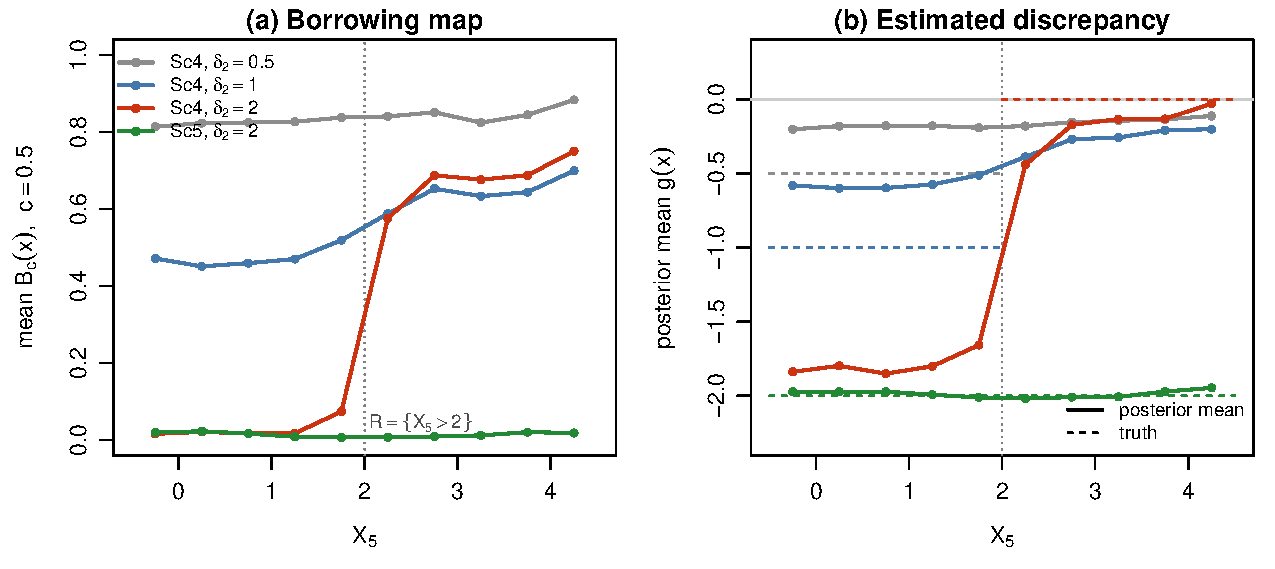
\includegraphics[width=0.74\textwidth]{inserts/lrc_fig_sc4_map.pdf}
  \vspace{-0.3em}
  \begin{block}{LRC-BART at target 100, first 40 replicates}
    At $\delta_2=2$ the map is $0.02$ outside $\mathcal R$ and $0.7$ inside, and $g$ is $-1.8$ and $-0.15$ against $-2$ and $0$; the transition occupies the unit around the boundary, learned from about four RCT controls per $0.1$ of $X_5$. At $\delta_2=1$ the estimate splits the shift ($-0.6$ / $-0.25$). Under Sc5 the map is $0.01$ everywhere.
  \end{block}
\end{frame}

\begin{frame}{What the Gaussian study shows}
  \begin{block}{When the sources agree}
    About $16\%$ less RMSE than the free-offset model, and more on the control surface; realized ESS $53$ against a prior ESS of $82$ and a ceiling of $127$.
  \end{block}
  \begin{block}{When they disagree everywhere}
    Abstention: realized ESS $1.6$ (Sc3) and $0.2$ (Sc5), bias about $0.04$ and $0.00$; the $0.04$ is $0.012$ above BART-PP with paired SE $0.001$, the price of a spike that is a Gaussian component and not a point mass.
  \end{block}
  \begin{alertblock}{When they disagree on a region}
    Found at $1.3$ residual SDs with a one-unit boundary transition and a shortfall of a tenth of the shift on each side, a sample-size limit that tuning did not remove. At one residual SD, near $d_{1/2}$, the method over-borrows: bias $-0.04$, coverage $0.89$, RMSE $0.223$ against $0.207$; the control surface in $\mathcal R$ is not better than BART-PP's ($0.824$ against $0.785$).
  \end{alertblock}
  \centering\footnotesize In Sc2 the ceiling falls from $127$ to $23$ under covariate shift, every absolute target is capped, and only the fractional ladder still moves.
\end{frame}

\begin{frame}{Survival outcomes}
  \centering
  \scriptsize
  \setlength{\tabcolsep}{4pt}
  \renewcommand{\arraystretch}{0.95}
  \begin{tabular}{lrrr|rrr|rrr}
    \toprule
    & \multicolumn{3}{c|}{Sc1, median ratio} & \multicolumn{3}{c|}{Sc3 $\rho=0$, median ratio} & \multicolumn{3}{c}{Sc3 $\rho=0$, RMST ratio} \\
    Method & Bias & RMSE & Pow & Bias & RMSE & Cov & Bias & RMSE & Cov \\
    \midrule
    AFT-NP  & 0.18 & 0.67 & 0.12 & 0.23 & 0.83 & 0.94 & $-$0.03 & 0.15 & 0.92 \\
    BART-NP & 0.26 & 0.51 & 0.46 & 0.19 & 0.57 & 0.90 & 0.06 & 0.17 & 0.92 \\
    BART-CP & 0.06 & 0.23 & 0.63 & 2.31 & 2.41 & 0.00 & 0.59 & 0.61 & 0.01 \\
    BART-PP & 0.03 & 0.35 & 0.25 & 0.04 & 0.45 & 0.91 & $-$0.01 & 0.14 & 0.92 \\
    C-BART  & 0.03 & 0.25 & 0.42 & 0.58 & 0.91 & 0.88 & 0.14 & 0.22 & 0.85 \\
    \textbf{LRC-BART (100)} & \textbf{0.05} & \textbf{0.31} & \textbf{0.34} & \textbf{0.15} & \textbf{0.56} & \textbf{0.94} & \textbf{0.03} & \textbf{0.15} & \textbf{0.94} \\
    \bottomrule
  \end{tabular}
  \vspace{0.3em}
  \begin{block}{Two readings}
    With $75$ controls and censoring the median ratio has a wide, skewed posterior whose mean is biased upward for every method; borrowing makes it usable (Sc1: RMSE $0.312$ against $0.345$, power $0.34$ against $0.25$ for BART-PP). Under unmeasured confounding LRC-BART abstains (realized ESS $2.3$) but its wider posterior, through the convex ratio, costs $0.11$ of median-ratio bias against BART-PP; on the RMST ratio the biases are $0.03$ and $-0.005$.
  \end{block}
\end{frame}

\begin{frame}[t]{The single-arm design}
  \footnotesize
  Trial contributes treated subjects only ($n_T=200$ Gaussian; $30$ or $200$ survival); the $300$ RWD controls are the sole control source; LRC-BART in single-arm mode with $w=1$.
  \begin{columns}[T,onlytextwidth]
    \column{0.49\textwidth}
      \begin{block}{No confounding}
        BART-CP and LRC-BART have Gaussian RMSE $0.16$; the survival RMST ratio at $n_T=30$ has RMSE $0.16$ to $0.19$ with coverage $0.92$ to $0.97$.
      \end{block}
    \column{0.49\textwidth}
      \begin{alertblock}{Measured confounding}
        Every method is biased: Gaussian ATE bias $1.68$ (LM-CP), $0.41$ (BART-CP), $0.42$ (LRC-BART); nothing in the data can reveal a discrepancy where the RWD does not cover the trial profiles.
      \end{alertblock}
  \end{columns}
  \vspace{0.3em}
  \begin{itemize}
    \item The single-arm ceiling is $27$ to $34$ under Sc2, so an absolute target of $100$ is capped and LRC-BART reduces to pooling; the fractional target still widens the interval (coverage $0.82$ to $0.99$).
    \item With $w<1$ the slab only adds prior noise, variance $(1-w)H_g\tau_1^2$: posterior SD $1.4$ on the ATE and $10$ to $34$ on the median ratio with the point estimate unchanged. Hence $w=1$ in single-arm mode.
    \item The hierarchical regressions with the stated hyperprior and no internal control are unusable (SD $8$ on the ATE).
  \end{itemize}
\end{frame}

\section{EloKRd application}
\begin{frame}{EloKRd and UCMM data}
  \begin{columns}[T,onlytextwidth]
    \column{0.48\textwidth}
      \begin{block}{EloKRd phase II trial}
        \begin{itemize}
          \item $n=30$, all received EloKRd
          \item 13 PFS events; 10 deaths
          \item 50\% high-risk cytogenetics; 30\% ASCT
        \end{itemize}
      \end{block}
    \column{0.48\textwidth}
      \begin{block}{UCMM registry control}
        \begin{itemize}
          \item $n=253$ after cohort restrictions
          \item Standard induction regimens
          \item Six harmonized baseline covariates
        \end{itemize}
      \end{block}
  \end{columns}
  \vspace{0.3em}
  \begin{alertblock}{A coding problem the calibration exposed}
    The non-Hispanic label differed between sources, so the earlier dummy coding predicted the 29 non-Hispanic trial patients from the 13-patient Hispanic registry stratum. The ESS ceiling at the trial profiles is $12.6$ (PFS) and $14.6$ (OS) under that coding and $63.7$ and $36.7$ under the harmonized one.
  \end{alertblock}
  \centering\footnotesize Estimand: standardized 5-year RMST ratio (neither trial median is reached). Kaplan--Meier: $1.015$ for PFS, $0.90$ for OS.
\end{frame}

\begin{frame}{EloKRd results: 5-year RMST ratio, posterior mean and 95\% interval}
  \centering
  \scriptsize
  \setlength{\tabcolsep}{6pt}
  \begin{tabular}{lcc}
    \toprule
    Harmonized coding & PFS & OS \\
    \midrule
    Kaplan--Meier, unadjusted & 1.01 (0.84, 1.22) & 0.90 (0.79, 1.03) \\
    Complete-pooling AFT & 0.87 (0.69, 1.06) & 0.80 (0.65, 0.94) \\
    Hierarchical AFT & 1.23 (0.74, 1.90) & 1.21 (0.77, 1.70) \\
    AFT-BART on UCMM, no discrepancy & 0.97 (0.79, 1.16) & 0.90 (0.78, 1.02) \\
    \midrule
    \textbf{LRC-BART, $\target=30$} & \textbf{0.97 (0.77, 1.23)} & \textbf{0.90 (0.77, 1.04)} \\
    LRC-BART, $\target=15$ & 0.99 (0.75, 1.40) & 0.91 (0.76, 1.11) \\
    LRC-BART, $0.9\times$ ceiling & 0.97 (0.79, 1.15) & 0.90 (0.77, 1.04) \\
    \midrule
    \textit{Earlier analysis, original coding:} MAP-AFT-BART, 30 & 1.08 (0.66, 16.4) & 0.97 (0.74, 4.77) \\
    \bottomrule
  \end{tabular}
  \vspace{0.3em}
  \begin{block}{Two readings}
    No nonparametric analysis supports a marginal EloKRd benefit ($P(\text{ratio}>1)$ of $0.37$ and $0.08$); the interval widens as the target falls, on a scale of tenths. The long upper tails of the earlier analysis were a property of its prior: with the discrepancy carried by a five-tree ensemble of pointwise variance $H_g\tau_0^2\approx0.07$, the PFS ratio at target $30$ has a $99.9$th percentile of $1.6$ over $8{,}000$ draws.
  \end{block}
\end{frame}

\begin{frame}{The local ESS map at the 30 trial profiles}
  \centering
  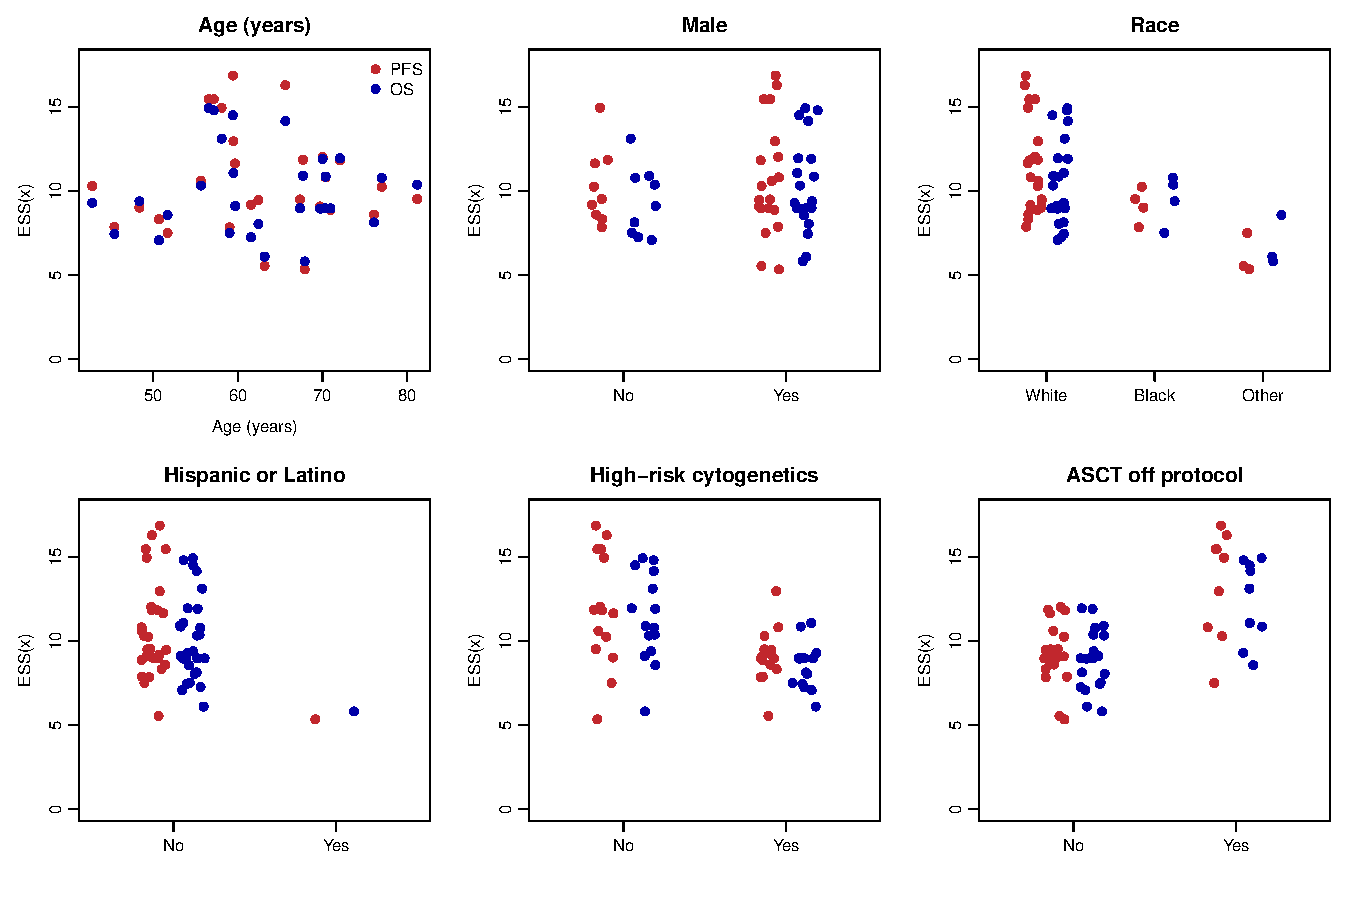
\includegraphics[height=0.58\textheight]{inserts/lrc_fig_ess_map.pdf}
  \vspace{-0.2em}
  \begin{block}{Reading the map}
    $\mathrm{ESS}(x)=\sigma_1^2/\{V_f(x)+H_g\tau_0^2\}$ ranges from $5$ to $17$ for PFS and $6$ to $15$ for OS: highest for White patients with ASCT and standard-risk cytogenetics, lowest for the one Hispanic patient, the Other/Unknown-race patients and the high-risk profiles without ASCT. A target of $30$ is spread thinly over the enrolled profiles.
  \end{block}
\end{frame}

\section{Takeaways}
\begin{frame}{Summary}
  \begin{enumerate}
    \item \textbf{Where borrowing is decided:} in the leaves of a discrepancy ensemble, so the tree prior chooses region by region and the choice is reported as a map.
    \item \textbf{Exactness:} every leaf marginal is closed-form; the sampler targets the exact posterior.
    \item \textbf{Calibration:} the prior ESS is defined at the estimand, has a ceiling equal to the information the external source carries about the trial population, and a target can be a fraction of that ceiling.
    \item \textbf{Guarantees:} bounded local influence, leaf resolution and map consistency, monotone well-posed calibration.
    \item \textbf{Evidence:} $16\%$ RMSE gain under agreement, abstention under global conflict, detection of a regional shift of $1.3$ SDs with a one-unit boundary transition, over-borrowing at a shift near the resolution.
  \end{enumerate}
\end{frame}

\begin{frame}{Limitations and next steps}
  \begin{itemize}
    \item Map results are conditional on the $g$ partitions and on $f$ fixed; nothing is proved about the posterior over partitions, which is where the boundary leak lives.
    \item A leaf-specific spike scale would let compatible regions differ, at the cost of conjugacy.
    \item Several external sources: one discrepancy ensemble per source with a common $w$; the ceiling becomes a sum.
    \item Binary and count outcomes; nonparametric survival BART in place of the AFT model.
    \item Prospective calibration to Type I error rate and power, with the map as a pre-specified diagnostic.
  \end{itemize}
  \vspace{0.5em}
  \begin{block}{Takeaway}
    LRC-BART borrows where the sources agree, abstains where they do not, and reports for each patient profile how much external information it used and how much was available.
  \end{block}
\end{frame}

\begin{frame}[allowframebreaks]{References}
  \scriptsize
  \bibliographystyle{unsrtnat}
  \bibliography{ref_lrcbart}
\end{frame}

\end{document}
